\documentclass[a4paper,12pt]{article}
\usepackage[latin1]{inputenc}
\usepackage[spanish]{babel}
\usepackage{amsmath}
\usepackage{graphicx}
\setlength{\textheight}{250mm}
\setlength{\textwidth}{165mm}
\setlength{\topmargin}{-15mm}
\setlength{\oddsidemargin}{0pt}
\pagestyle{empty}

\begin{document}

\def\bm#1{{\mbox{\boldmath $#1$}}}
\def\eqdef{\buildrel \rm def \over =}
\def\signo{\mathop{\rm signo}\nolimits}

\mbox{}\vspace*{-20mm}

\begin{center}
{\small\sc Escuela T�cnica Superior de Ingenieros de Caminos, Canales y Puertos (Madrid)}\\*[4mm]
{\Large\bf M�todo de los Elementos Finitos}\\*[4mm]
Ejercicio 4: Tecnolog�a de elementos.
\end{center}

% \vspace{4mm}

% ENUNCIADO
La estructura de la figura, cuyas dimensiones est�n indicadas en la misma,
est� fabricada con un material cuyas propiedades mec�nicas son
$E=20.5$ GPa y $\nu=0.23$. Las cargas aplicadas tienen todas el mismo
valor $F=1000$ kN. Las condiciones de contorno a aplicar son las
correspondientes a que los planos $OXY$, $OXZ$ y $OYZ$ sean planos de
simetr�a.

La discretizaci�n a considerar son $2$ elementos en el espesor y $20 \times 20$
elementos en las caras verticales (situadas fuera de los planos
coordenados). Para resolver el problema se utilizar�n elementos hexa�dricos
de $8$ nodos con formulaciones en desplazamientos, mixta y
deformaciones mejoradas supuestas (modos incompatibles).

{\em NOTA:En el sitio de la asignatura en Moodle se cargar� el fichero con los contornos de movimientos en direcci�n $Z$ obtenido con los elementos
de deformaciones supuestas mejoradas}.

\vspace{5mm}
\begin{center}
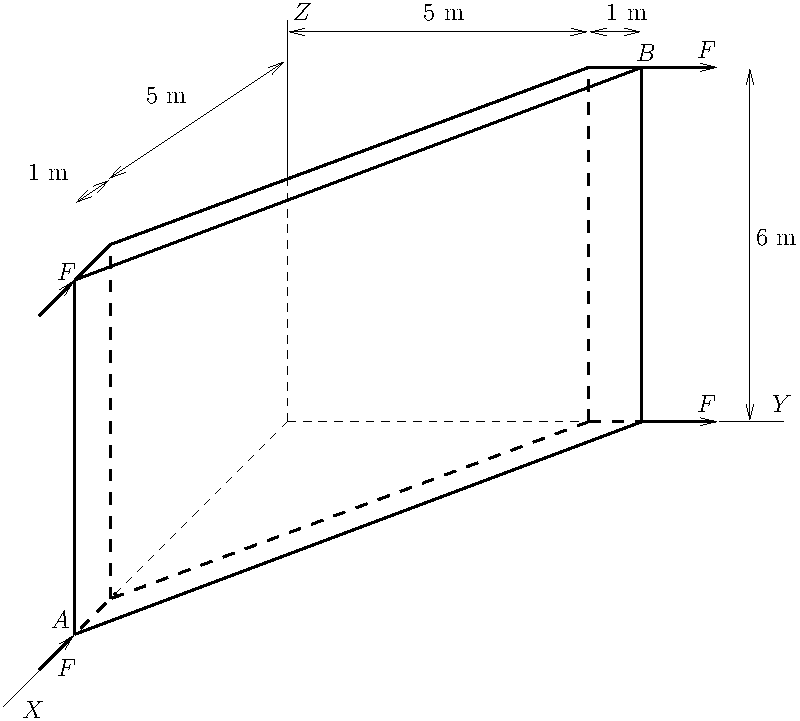
\includegraphics[width=0.7\textwidth]{ejerc4}
\end{center}

\end{document}
